\documentclass[italian,a4paper]{article}
\usepackage[tight,nice]{units} %unità di misura
\usepackage{babel,amsmath,amssymb,amsthm,graphicx,url}
\usepackage[text={5.5in,9in},centering]{geometry}
\usepackage[utf8x]{inputenc}
\usepackage[T1]{fontenc}
\usepackage{ae,aecompl}
\usepackage[footnotesize,bf]{caption}
\usepackage[usenames]{color}
\usepackage{textcomp}
\usepackage{gensymb}
\usepackage{pstricks}
\frenchspacing
\pagestyle{plain}
%------------- eliminare prime e ultime linee isolate
\clubpenalty=9999%
\widowpenalty=9999
%--- definizione numerazioni
\renewcommand{\theequation}{\thesection.\arabic{equation}}
\renewcommand{\thefigure}{\arabic{figure}}
\renewcommand{\thetable}{\arabic{table}}
\addto\captionsitalian{%
\renewcommand{\figurename}%
{Grafico}%
}
%
%------------- ridefinizione simbolo per elenchi puntati: en dash
%\renewcommand{\labelitemi}{\textbf{--}}
\renewcommand{\labelenumi}{\textbf{\arabic{enumi}.}}
\setlength{\abovecaptionskip}{\baselineskip}   % 0.5cm as an example
\setlength{\floatsep}{2\baselineskip}
\setlength{\belowcaptionskip}{\baselineskip}   % 0.5cm as an example
%--------- comandi insiemi numeri complessi, naturali, reali e altre abbreviazioni
\renewcommand{\leq}{\leqslant}
%--------- porzione dedicata ai float in una pagina:
\renewcommand{\textfraction}{0.05}
\renewcommand{\topfraction}{0.95}
\renewcommand{\bottomfraction}{0.95}
\renewcommand{\floatpagefraction}{0.35}
\setcounter{totalnumber}{5}
%---------
%
%---------
\begin{document}
\title{Relazione di laboratorio: transistor}
\author{\normalsize Ilaria Brivio (582116)\\%
\normalsize \url{brivio.ilaria@tiscali.it}%
\and %
\normalsize Matteo Abis (584206)\\ %
\normalsize \url{webmaster@latinblog.org}
\and %
\normalsize Lorenzo Rossato (579393)\\ %
\normalsize \url{supergiovane05@hotmail.com}}
\date{\today}
\maketitle
%------------------
\noindent
Abbiamo realizzato il circuito in figura~\ref{fig:circuito} con un transistor BC107B e due
resistenze $R_b = \unit[150]{k\ohm}$ e $R_c = \unit[1]{k\ohm}$. I
valori misurati sono $R_b = \unit[149.3 \pm 0.75]{k\ohm}$ e $R_c = \unit[1.008 \pm
0.005]{k\ohm}$, dal il multimetro T110B, fondo scala
rispettivamente $\unit[200]{k\ohm}$ e $\unit[2]{k\ohm}$. In $A$ è collegato
il generatore di tensione continua, in $V_0$ la tensione continua in ingresso
è fissata a $\unit[15.03]{V}$.
\begin{figure}[h]
    \caption{Rappresentazione schematica del circuito realizzato}
    \label{fig:circuito}
    \begin{center}
        \psset{unit=1in,cornersize=absolute,dimen=middle}%
\begin{pspicture}(-1.395,-0.9625)(0.383333,1.254722)%
% dpic version 16.Jan.09 for PSTricks 0.93a or later
\psset{linewidth=0.8pt}%
\psset{linewidth=0.8pt}%
\makeatletter\@ifundefined{MPSTPatchA}{\def\psbezier@ii{\addto@pscode{%
\ifshowpoints true \else false \fi\tx@OpenBezier%
\ifshowpoints\tx@BezierShowPoints\fi}\end@OpenObj}%
\global\def\MPSTPatchA{}}{}\makeatother%
\psset{arrowsize=1.1pt 4,arrowlength=1.64,arrowinset=0}%
\psline(0,0)(0,0.15)
(0,0.15)(-0.01107,0.15)
\psline(0,0.6)(0,0.45)
(0,0.45)(-0.01107,0.45)
\psline(-0.2,0.2)(-0.2,0.4)
\psline(-0.325,0.3)(-0.2,0.3)
\psline(0,0.15)(-0.2,0.24)
\psline[arrowsize=0.055556in 0,arrowlength=1.5,arrowinset=0]{<-}(-0.05,0.1725)(-0.15,0.2175)
\psline(0,0.45)(-0.2,0.36)
\psline(0,0.6)(0,0.775)
(0,0.775)(-0.041667,0.795833)
(-0.041667,0.795833)(0.041667,0.8375)
(0.041667,0.8375)(-0.041667,0.879167)
(-0.041667,0.879167)(0.041667,0.920833)
(0.041667,0.920833)(-0.041667,0.9625)
(-0.041667,0.9625)(0.041667,1.004167)
(0.041667,1.004167)(0,1.025)
(0,1.025)(0,1.2)
\uput{0.501875ex}[r](0.041667,0.9){\rlap{$ R_c$}}
\pscircle[fillstyle=solid,fillcolor=black](0,0.6){0.02}
\uput{0.501875ex}[r](0.02,0.6){\rlap{$ V_\text{out}$}}
\pscircle[fillstyle=solid,fillcolor=black](0,1.2){0.02}
\uput{0.501875ex}[u](0,1.22){$ +\unit[15]{V}$}
\psline(-0.325,0.3)(-0.775,0.3)
\psline(-0.775,0.3)(-0.775,0.6)
\psline(-0.775,0.6)(-0.775,0.775)
(-0.775,0.775)(-0.816667,0.795833)
(-0.816667,0.795833)(-0.733333,0.8375)
(-0.733333,0.8375)(-0.816667,0.879167)
(-0.816667,0.879167)(-0.733333,0.920833)
(-0.733333,0.920833)(-0.816667,0.9625)
(-0.816667,0.9625)(-0.733333,1.004167)
(-0.733333,1.004167)(-0.775,1.025)
(-0.775,1.025)(-0.775,1.2)
\uput{0.501875ex}[r](-0.733333,0.9){\rlap{$ R_1$}}
\pscircle[fillstyle=solid,fillcolor=black](-0.775,1.2){0.02}
\uput{0.501875ex}[u](-0.775,1.22){$ +\unit[15]{V}$}
\psline(-0.775,0.3)(-0.775,0)
\psline(-0.775,0)(-0.775,-0.325)
(-0.775,-0.325)(-0.733333,-0.345833)
(-0.733333,-0.345833)(-0.816667,-0.3875)
(-0.816667,-0.3875)(-0.733333,-0.429167)
(-0.733333,-0.429167)(-0.816667,-0.470833)
(-0.816667,-0.470833)(-0.733333,-0.5125)
(-0.733333,-0.5125)(-0.816667,-0.554167)
(-0.816667,-0.554167)(-0.775,-0.575)
(-0.775,-0.575)(-0.775,-0.9)
\uput{0.501875ex}[r](-0.733333,-0.45){\rlap{$ R_2$}}
\psline(-0.691667,-0.9)(-0.858333,-0.9)
\psline(-0.719444,-0.93125)(-0.830556,-0.93125)
\psline(-0.739286,-0.9625)(-0.810714,-0.9625)
\psline(-0.775,0.3)(-1.05,0.3)
\psline(-1.05,0.383333)(-1.05,0.216667)
\psline(-1.1,0.383333)(-1.1,0.216667)
\psline(-1.1,0.3)(-1.375,0.3)
\uput{0.501875ex}[u](-1.075,0.383333){$ C_1$}
\pscircle[fillstyle=solid,fillcolor=black](-1.375,0.3){0.02}
\uput{0.501875ex}[d](-1.375,0.28){$ V_\text{in}$}
\psline(0,0)(-0,-0.1)
(-0,-0.1)(0.041667,-0.120833)
(0.041667,-0.120833)(-0.041667,-0.1625)
(-0.041667,-0.1625)(0.041667,-0.204167)
(0.041667,-0.204167)(-0.041667,-0.245833)
(-0.041667,-0.245833)(0.041667,-0.2875)
(0.041667,-0.2875)(-0.041667,-0.329167)
(-0.041667,-0.329167)(0,-0.35)
(0,-0.35)(0,-0.45)
\uput{0.501875ex}[l](-0.125,-0.225){\llap{$ R_{e1}$}}
\psline(0,-0.45)(-0,-0.55)
(-0,-0.55)(0.041667,-0.570833)
(0.041667,-0.570833)(-0.041667,-0.6125)
(-0.041667,-0.6125)(0.041667,-0.654167)
(0.041667,-0.654167)(-0.041667,-0.695833)
(-0.041667,-0.695833)(0.041667,-0.7375)
(0.041667,-0.7375)(-0.041667,-0.779167)
(-0.041667,-0.779167)(0,-0.8)
(0,-0.8)(0,-0.9)
\uput{0.501875ex}[l](-0.125,-0.675){\llap{$ R_{e2}$}}
\psline(0.083333,-0.9)(-0.083333,-0.9)
\psline(0.055556,-0.93125)(-0.055556,-0.93125)
\psline(0.035714,-0.9625)(-0.035714,-0.9625)
\psline(0,-0.45)(0.3,-0.45)
\psline(0.3,-0.45)(0.3,-0.65)
\psline(0.216667,-0.65)(0.383333,-0.65)
\psline(0.216667,-0.7)(0.383333,-0.7)
\psline(0.3,-0.7)(0.3,-0.9)
\uput{0.501875ex}[ur](0.325,-0.675){\rlap{$ C_2$}}
\psline(0.383333,-0.9)(0.216667,-0.9)
\psline(0.355556,-0.93125)(0.244444,-0.93125)
\psline(0.335714,-0.9625)(0.264286,-0.9625)
\end{pspicture}%

    \end{center}
\end{figure}\\
Con un valore di $V_a = \unit[5.09]{V}$
abbiamo misurato con il multimetro $V_c = \unit[4.45]{V}$ e $V_b =
\unit[0.668]{V}$. Da cui si può ricavare una prima stima di $\beta$.
\begin{equation*}
    \beta_0 = \dfrac{V_{0} - V_c}{V_a - V_b}\dfrac{R_b}{R_c} = 350
\end{equation*}
Con questo $\beta_0$ abbiamo stimato quali valori di $V_a$ impostare per ottenere
correnti di collettore di 2, 5, 8 e \unit[10]{mA}. 
Infatti $I_c$ vale:
\begin{equation*}
    I_c = \unit[\dfrac{V_a - 0.6}{150}350]{mA}
\end{equation*}
Da cui si ricavano i valori opportuni di $V_a$, che risultano (vedi
tabella) 1.5, 2.7, 4.0 e \unit[4.9]{V}.
Abbiamo dunque misurato i corrispondenti valori di $V_b$ e $V_c$.
Da ogni terna di valori si può stimare $\beta$ con la stessa formula
scritta sopra. Nella tabella è riportato come riferimento anche il calcolo
delle correnti di base e collettore.

Non abbiamo calcolato le tolleranze sulle determinazioni del parametro
$\beta$ perch\'e esso dipende da molti fattori e può variare
molto anche per lo stesso transistor, a seconda delle condizioni di
lavoro. Al contrario le tolleranze sarebbero dell'1.5\%, essendo i
potenziali e le resistenze calcolate con scale diverse sul multimetro, e
quindi comunque poco significative. Poich\'e però nelle esperienze successive servirà un riferimento
sul fattore di amplificazione di questo transistor, calcoliamo la media
aritmetica, associandovi come errore massimo la semidispersione di questi dati.
\begin{equation*}
    \bar\beta = 365\pm11
\end{equation*}
\begin{table}[h]\caption{Dati raccolti per i potenziali ai terminali A,B e
    C, in Volt, correnti in \unit[]{mA} e relativi valori di $\beta$ calcolati.}
    \centering
    \begin{tabular}{*6c}
$V_a$ & $V_b$ & $V_c$ & $I_b$ & $I_c$ & $\beta$ \\\hline
1.51 & 0.636 & 12.81 & 0.006 & 2.20 & 374\\
2.72 & 0.647 & 9.76 & 0.014 & 5.23 & 376\\
4.04 & 0.657 & 6.66 & 0.023 & 8.30 & 366\\
4.90 & 0.667 & 4.86 & 0.028 & 10.09 & 355\\
5.09 & 0.668 & 4.45 & 0.030 & 10.50 & 354\\
\end{tabular}
    \end{table}\\
    
Ora $V_{\text{in}}$ è un segnale:
\begin{table}[h]
    \centering
    \begin{tabular}{rl}
        forma: & onda quadra\\
        frequenza: & \unit[10.40]{kHz}\\
        ampiezza pp: & \unit[5]{V}\\
        valor medio: & \unit[2.5]{V}
    \end{tabular}
\end{table}\\
La resistenza $R_{\text{c}}$ è ancora \unit[$1$]{k\ohm} mentre $R_{\text{b}}$ vale \unit[330]{k\ohm}. L'andamento
dell'ingresso e dell'uscita in funzione del tempo per la durata di un
periodo è riportato in figura~\ref{fig:vinvout1} e~\ref{fig:vinvout2}. Le
figure non si riferiscono ai dati qui
riportati in quanto sono state realizzate in altra data, e quindi in
condizioni leggermente diverse, sebbene il più possibile fedeli alle
istruzioni registrate sul \emph{diario di bordo}.
\begin{figure}[h]
    \begin{center}
    \caption{Segnale in salita nell'oscilloscopio.}
    \label{fig:vinvout1}
        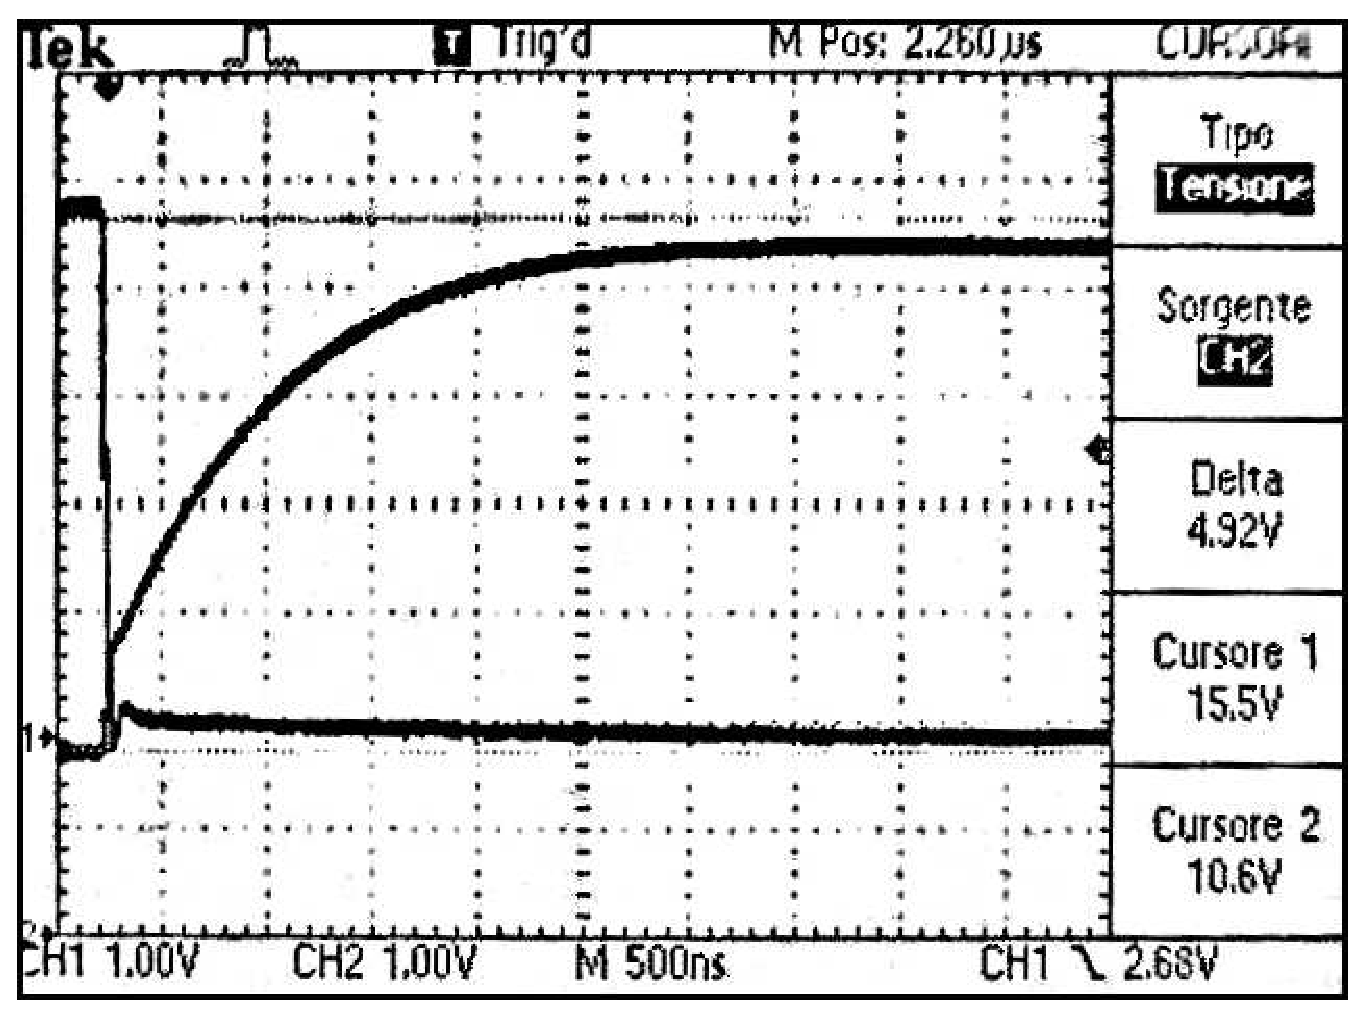
\includegraphics[width=0.7\textwidth]{salita.eps}
    \end{center}
\end{figure}
\begin{figure}[h]
    \begin{center}
    \caption{Segnale in discesa nell'oscilloscopio.}
    \label{fig:vinvout2}
        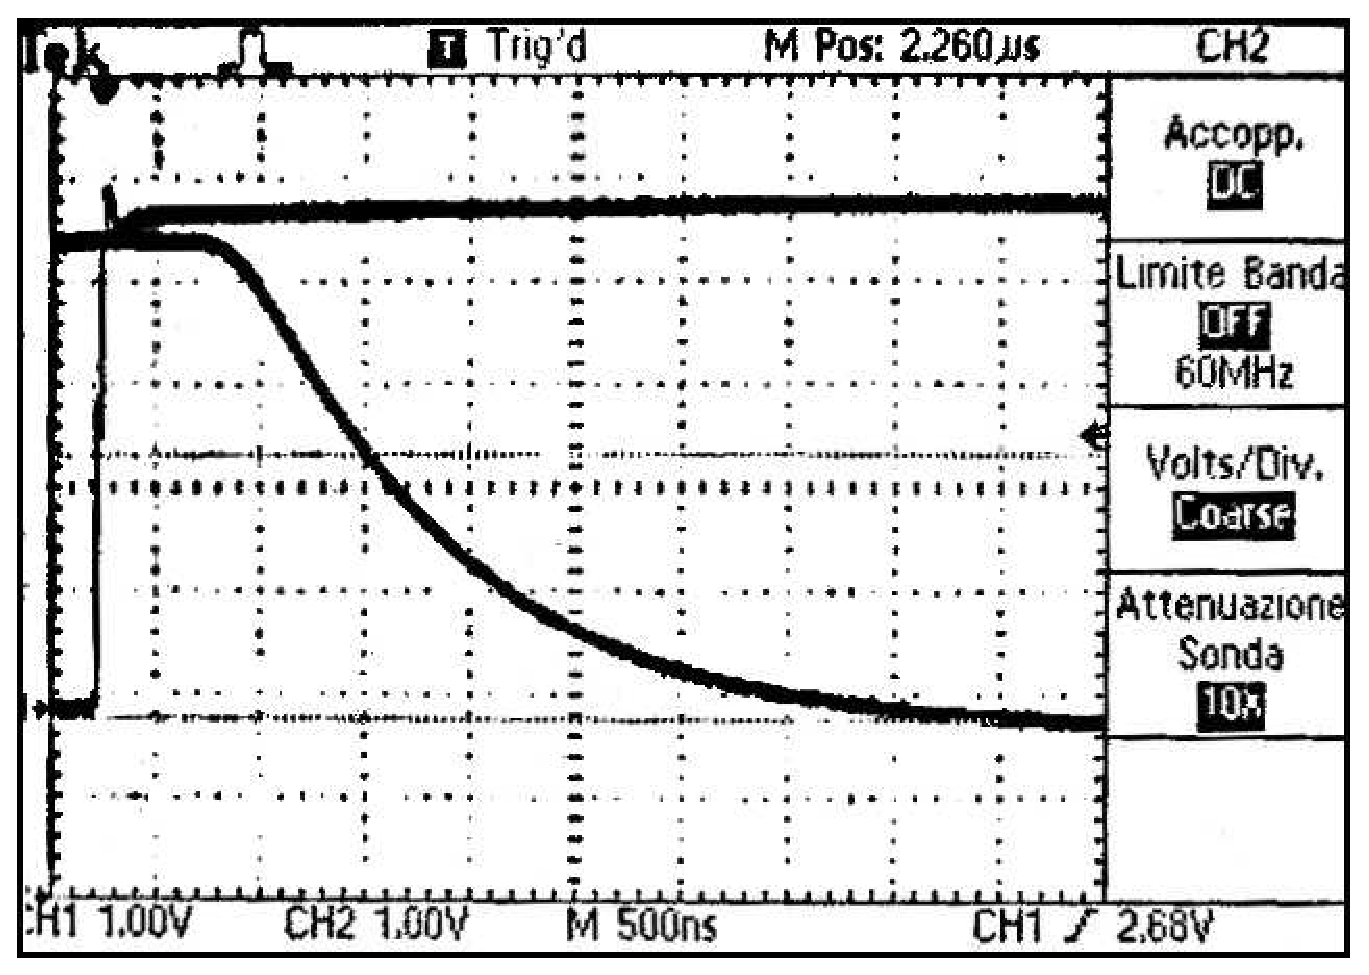
\includegraphics[width=0.7\textwidth]{discesa.eps}
    \end{center}
\end{figure}\\
Al segnale in $V_{\text{out}}$ corrisponde un valore di
$\Delta V = \unit[4.48]{V}$. Definito il tempo di salita di un segnale
il tempo impiegato per passare dal $10 \%$ al $90 \%$ del suo valore
finale (ugualmente per la discesa), abbiamo $10 \% \Delta V =
\unit[0.45]{V}$ e $90\% \Delta V = \unit[4.03]{V}$ a cui corrisponde una
differenza di tempo di:
\begin{table}[h]
    \centering
    \begin{tabular}{*4c}
        &  t & V/div & T/div\\
        salita & \unit[1740]{ns} & \unit[1] {V} & \unit[500]{ns}\\
    discesa & \unit[2720]{ns} & \unit[1]{V} & \unit[500]{ns}\\
\end{tabular} \end{table}\\

Si vuole infine calcolare il valore minimo della resistenza di collettore
che manda il transistor in saturazione, quando $V_{\text{out}}$
raggiunge il valore di circa \unit[0.2]{V}.  Abbiamo una stima
di $\beta$ dall'esperimento precedente, quindi diciamo $I_{\text{c}}=
\beta I_{\text{b}}= 365 \cdot \unit[13]{\micro A}= \unit[4.7]{mA}$;
dall'equazione $V_{\text{e}} - I_{\text{c}}R = \unit[0.2]{V}$ si
ottiene esplicitando la resistenza una stima di $R = {14.8}/{4.7}=
\unit[3.15]{k\ohm}$. Per verificare tale stima abbiamo impiegato un
potenziometro e abbiamo misurato a quale valore della resistenza il segnale
in uscita risultava appiattito su circa \unit[0.2]{V}. La resistenza risulta
essere $R =\unit[3.30\pm0.02]{k\ohm} $ e $V_{\text{c}}= \unit[0.192]{V}$, in buon
accordo con quanto previsto.
\end{document}
